\documentclass[11pt]{article}
\usepackage{polski}
\usepackage[utf8]{inputenc}
\usepackage{amsthm}
\usepackage{listings}
\usepackage{hyperref}
\usepackage{graphicx}


\newtheoremstyle{note}% style name 
{2ex}% above space 
{2ex}% below space 
{}% body font 
{}% indent amount 
{\scshape}% head font 
{}% post head punctuation 
{\newline}% post head punctuation 
{}% head spec 

\theoremstyle{note}
\newtheorem{theorem}{Twierdzenie}[section]

\newtheorem{definition}[theorem]{Definicja}
%Gummi|065|=)
\title{\textbf{3SAT - algorytm genetyczny vs DPLL}
\large Raport projektu z przedmiotu Inteligencja Obliczeniowa}
\author{Krzysztof Łozowski \\ 255157}
\date{24 stycznia 2018}

\begin{document}

\maketitle

\section{Wprowadzenie}
Celem projektu jest zaprezentowanie i porównanie czasów działania algorytmu genetycznego oraz algorytmu DPLL dla zagadnienia 3SAT. \\
Przed rozpoczęciem analizy problemu podane zostaną podstawowe definicje dotyczące wspomnianego zagadnienia.

\begin{definition}[KPN]
Formuła $\phi$ jest w koniunkcyjnej postaci normalnej jeśli jest ona koninkcją klauzul, z których każda jest alternatywą literałów, tzn. jest ona postaci
  \begin{displaymath}
    (p_{11} \vee \ldots \vee p_{1k_{1}}) \ \wedge \ (p_{21} \vee \ldots \vee p_{2k_{2}}) \ \wedge \ldots \wedge \ (p_{n1} \vee \ldots \vee p_{nk_{n}})
  \end{displaymath}
gdzie każde $p_{ij}$ jest literałem.
\end{definition}

\begin{definition}[k-SAT]
  Formuła logiczna postaci KPN, w której każda klauzula składa się z nie więcej niż $k$ literałów.
\end{definition}

\noindent Zagadnienia $1$-SAT oraz $2$-SAT można rozwiązać w deterministycznym czasie wielomianowym $P$. \\
Rozważane przez nas zagadnienie $3$-SAT jest już z kolei NP-zupełne, czyli takie, że każdy problem z klasy NP jest do niego redukowalny przy pomocy redukcji w czasie wielomianowym. \\
W projekcie rozważane są jedynie formuły rozwiązywalne, ponieważ jego głównym założeniem jest porównanie czasów działania algorytmów a nie problem rozwiązywalności formuł. \\

\noindent
Repozytorium projektu dostępne jest pod adresem \\\url{https://github.com/lozovsky/GAvsDPLL}.


\newpage
\section{Algorytm Genetyczny}
W projekcie użyty został algorytm genetyczny, którego implementacja w języku \textbf{R} znajduje się w paczce \textbf{genalg}.
\begin{lstlisting}[language=R]
	install.packages("genalg")
\end{lstlisting}
Na początku istotnym problemem był dobór odpowiednich parametrów dla algorytmu. 

\subsection{Dane i ich obróbka}
W celu doboru odpowiednich parametrów zdecydowałem się na porównanie spełnialności skryptu dla wielu formuł. \\
Wybraną paczką danych została paczka o nazwie \textbf{CBS\_k3\_n100\_m403\_b10} dostępna pod adresem \url{http://www.cs.ubc.ca/~hoos/SATLIB/benchm.html}. Pliki te znajdują się w folderze B403. \\
\subsubsection{Wstępna obróbka danych}


Następną czynnością do wykonania była obróbka tych danych. Proces ten został podzielony na następujące etapy:
\begin{enumerate}
  \item Usunięcie zbędnych wierszy z plików
  \item Usunięcie liczby 0 z końca każdego wiersza
  \item Podział danych na kolumny z indeksami oraz wartościami logicznymi
  \item Zamiana minusów na poprawione wartości logiczne
\end{enumerate}

Dwa pierwsze podpunkty związane były stricte z operacjami na plikach, a ponieważ było ich aż 1000, to ręczna obróbka każdego z nich zajęłaby zbyt wiele czasu. \\
Można było jednak zauważyć, że w każdym z tych plików do wykonania były dokładnie te same operacje, więc przy użyciu komend w edytorze VIM:
\begin{lstlisting}[language=bash]
	:set hidden
	:args *
	:argdo %s/  0//g
	:argdo 1,4d
	:wa
\end{lstlisting}

\noindent Pliki te miały zagwarantowaną rozwiązywalność. W celu wygenerowania mniejszych plików (wprawdzie bez gwarancji rozwiązywalności, lecz zapewne część będzie rozwiązywalna), zostały stworzone odpowiednie foldery
\begin{lstlisting}[language=bash]
$ echo B10/ B20/ B50/ B100/ B200/ B300/ | xargs -n 1 cp -rf B403/
\end{lstlisting}
a następnie przeprowadzono redukcję do odpowiedniej liczby literałów
\begin{lstlisting}[language=bash]
	:set hidden
	:args B10/*
	:argdo 11,403d
	:wa
\end{lstlisting}
Operacje dla pozostałych folderów były niemal identyczne, nie ma sensu powielać poleceń.

\subsubsection{Dalsza obróbka danych w skrypcie}
Aby dane nadawały się do użytku dla funkcji fitness, należało zrobić jeszcze dwie rzeczy:
\begin{enumerate}
\item Odseparować indeks zmiennej od jej wartości logicznej 
\item Pozbyć się minusa przy numerze indeksu, jednocześnie zmieniając wartość logiczną tej zmiennej na przeciwną
\end{enumerate}
Za pierwszą z nich odpowiada funkcja $separateIndexFromValue$:
\begin{lstlisting}[language=R]
separateIndexFromValue <- function(data_frame_to_clear){
  number_of_rows = length(data_frame_to_clear[,1])
  DT <- data.frame(
                   V1_index = data_frame_to_clear[,1],
                   V1_value = matrix(1,number_of_rows),
                   V2_index = data_frame_to_clear[,2],
                   v2_value = matrix(1,number_of_rows),
                   V3_index = data_frame_to_clear[,3],
                   V3_value = matrix(1,number_of_rows)
                   )
  return(DT)
}
\end{lstlisting}
\newpage
\noindent
Za drugą natomiast odpowiada funkcja $fixMinusAndValue$:
\begin{lstlisting}[language=R]
separateIndexFromValue <- function(data_frame_to_clear){
fixMinusAndValue <- function(DT){
  for (i in 1:length(DT[,1])){
    for (j in seq(1, 6, 2)){
      if (DT[i,j] < 0){ 
        DT[i,j] = abs(DT[i,j])
        DT[i,j+1] = 0 
      }   
    }   
  }
  return(DT)
}
\end{lstlisting}
Obie funkcje wywoływane są przez funkcję $cleanData$, dzięki czemu dane są gotowe do pracy z algorytmem genetycznym.
\begin{lstlisting}[language=R]
cleanData <- function(data_frame_to_clear){
  DT = separateIndexFromValue(data_frame_to_clear)
  DT = fixMinusAndValue(DT)
}
\end{lstlisting}
\subsection{Funkcja fitness}
Chcemy, by funkcja fitness przyporządkowywała lepszym wynikom coraz mniejsze wartości. 
Każdy literał, który jest prawdziwy zmniejsza ocenę o 1. \\
Najlepsza ocena możliwa do uzyskania równa się liczbie literałów danej formuły.
\begin{lstlisting}[language=R]
fitnessFunc <- function(chromosome = c(), DT = cleanDataFrame){
  value = 0 
  number_of_rows = length(DT[,1])
  for (i in 1:number_of_rows){
      if (chromosome[DT[i,1]] == DT[i,2] || chromosome[DT[i,3]] == DT[i,4] 
       || chromosome[DT[i,5]] == DT[i,6]){
        value = value -1
      }   
  }

  return(value)
}
\end{lstlisting}
\subsection{Dobór parametrów}
Wszystkie logi dostępne w repozytorium na GitHubie
\subsubsection{10 literałów}
Dla niewielkiej liczby literałów wystarczyły również stosunkowo niewielkie parametry  $Population Size=10$ oraz $NumberOfGenerations=20$. \\
\begin{lstlisting}[language=R]
[1] "Liczba prawidlowych wynikow"
[1] 964
[1] "Liczba nieprawidlowych wynikow"
[1] 36
[1] "Sredni czas wykonania"
[1] 0.2175534 (s)
\end{lstlisting}
Występowanie wyników nieprawidłowych może być spowodowane skracaniem oryginalnych formuł. \\
Dobrane parametry są zadowalające.

\subsubsection{20 literałów}
Population Size = 10, Number of Generations = 20
\begin{lstlisting}[language=R]
[1] "Liczba prawidlowych wynikow"
[1] 881
[1] "Liczba nieprawidlowych wynikow"
[1] 119
[1] "Sredni czas wykonania"
[1] 0.332041 (s)
\end{lstlisting}
\noindent\rule{13cm}{0.4pt}\\
Population Size = 20, Number of Generations = 20
\begin{lstlisting}[language=R]
[1] "Liczba prawidlowych wynikow"
[1] 998
[1] "Liczba nieprawidlowych wynikow"
[1] 2
[1] "Sredni czas wykonania"
[1] 0.7549588 (s)
\end{lstlisting}
Czas wykonania wzrasta ponad dwukrotnie, lecz liczba zadowalających wyników jest niemal perfekcyjna.
\newpage
\subsubsection{50 literałów}
Population Size = 10, Number of Generations = 20
\begin{lstlisting}[language=R]
[1] "Liczba prawidlowych wynikow"
[1] 414
[1] "Liczba nieprawidlowych wynikow"
[1] 586
[1] "Sredni czas wykonania"
[1] 0.7309625 (s)
\end{lstlisting}
\noindent\rule{13cm}{0.4pt}\\
Population Size = 50, Number of Generations = 20
\begin{lstlisting}[language=R]
[1] "Liczba prawidlowych wynikow"
[1] 991
[1] "Liczba nieprawidlowych wynikow"
[1] 9
[1] "Sredni czas wykonania"
[1] 3.221467 (s)
\end{lstlisting}
Znaczące zwiększenie zwiększa precyzję jak i czas wykonania skryptu.

\subsubsection{100 literałów}
Population Size = 10, Number of Generations = 20
\begin{lstlisting}[language=R]
[1] "Liczba prawidlowych wynikow"
[1] 39
[1] "Liczba nieprawidlowych wynikow"
[1] 961
[1] "Sredni czas wykonania"
[1] 1.244902 (s)
\end{lstlisting}
\noindent\rule{13cm}{0.4pt}\\
Population Size = 50, Number of Generations = 20
\begin{lstlisting}[language=R]
[1] "Liczba prawidlowych wynikow"
[1] 560
[1] "Liczba nieprawidlowych wynikow"
[1] 440
[1] "Sredni czas wykonania"
[1] 5.719035 (s)
\end{lstlisting}
Proponowany Population Size = 100

\subsubsection{200 literałów}
Population Size = 10, Number of Generations = 20
\begin{lstlisting}[language=R]
[1] "Liczba prawidlowych wynikow"
[1] 0
[1] "Liczba nieprawidlowych wynikow"
[1] 10000
[1] "Sredni czas wykonania"
[1] NaN
\end{lstlisting}
Średni czas jest liczony jedynie dla prawidłowych wyników\\
\noindent\rule{13cm}{0.4pt}\\
Population Size = 50, Number of Generations = 20
\begin{lstlisting}[language=R]
[1] "Liczba prawidlowych wynikow"
[1] 1
[1] "Liczba nieprawidlowych wynikow"
[1] 999
[1] "Sredni czas wykonania"
[1] 10.602 (s)
\end{lstlisting}
\noindent\rule{13cm}{0.4pt}\\
Population Size = 150, Number of Generations = 50
\begin{lstlisting}[language=R]
[1] "Liczba prawidlowych wynikow"
[1] 102
[1] "Liczba nieprawidlowych wynikow"
[1] 153
[1] "Sredni czas wykonania"
[1] 1.2398 (mins)
\end{lstlisting}
Ze względu na znaczny wzrost czasu wykonania (głównie przez zwiększenie liczby generacji) zmniejszona została liczba testowanych formuł. \\ Liczba wyników prawidłowych pozostaje niezadowalająca. \\
Proponowane: Population Size = 300, Number of Generations = 100

\newpage
\subsubsection{300 literałów}
Population Size = 10, Number of Generations = 20
\begin{lstlisting}[language=R]
[1] "Liczba prawidlowych wynikow"
[1] 0
[1] "Liczba nieprawidlowych wynikow"
[1] 1000
[1] "Sredni czas wykonania"
[1] NaN
\end{lstlisting}
\noindent\rule{13cm}{0.4pt}\\
Population Size = 150, Number of Generations = 50
\begin{lstlisting}[language=R]
[1] "Liczba prawidlowych wynikow"
[1] 2
[1] "Liczba nieprawidlowych wynikow"
[1] 184
[1] "Sredni czas wykonania"
[1] 2.0705 (mins)
\end{lstlisting}
O wiele za małe wartości testowe. \\
Proponowane: Population Size = 450, Number of Generations = 100

\subsubsection{403 literały}
Population Size = 150, Number of Generations = 50
\begin{lstlisting}[language=R]
[1] "Liczba prawidlowych wynikow"
[1] 0
[1] "Liczba nieprawidlowych wynikow"
[1] 143
[1] "Sredni czas wykonania"
[1] 2.0705 (mins)
\end{lstlisting}
O wiele za małe wartości testowe. \\
Proponowane: Population Size = 600, Number of Generations = 100



\newpage
\section{DPLL}
Użyta implementacja algorytmu dostępna jest pod adresem \\\url{https://github.com/ashwinkachhara/3dpll}. \\
Użyty język: Python

\section{Porównanie}
Dla obu algorytmów użyto tych samych danych testowych. \\
Otrzymano następujące wyniki:\\

\begin{tabular}{c|r|rll}
Literały & \multicolumn{1}{l|}{GA} & \multicolumn{1}{l}{DPLL} &  &  \\ \cline{1-3}
10       & 0.140135[s]              &           0.022[s]               &  &  \\
20       & 1.36323[s]                &                 0.026[s]        &  &  \\
50       & 18.94206[s]               &                         0.039[s] &  & \\
100      & 39.86838[s]                &           0.108[s]               &  &  \\
200      & 1.831965[min]                &               4.287[s]           &  &  \\
300      & 4.528744[min]                &              0.995[s]            &  &  \\
400      & 16.28383[min]                &               7[min]17.359[s]           &  &  \\
403      & 12.86907[min]                &                 13[min]12.759[s]         &  &  
\end{tabular}

\begin{figure}[htp]
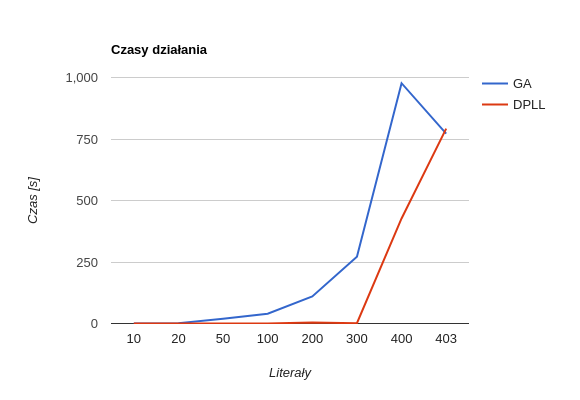
\includegraphics[scale=0.64]{graph1.png}
\end{figure}


\end{document}
